\subsection{Filters}
%\todo{jan: verify post proofreading}
We have now established that filters are stand-alone programs that
takes input, performs some projection and outputs the result. 
This leads us to a more detailed description of the filters
developed for this thesis. 

The filters can be combined to make a whole; though naturally some
combinations makes more sense than others. For example it generally
makes sense to put filters that remove unnecessary information early
in the stream, to reduce the input data-sizes for downstream filters.

%% \todo[inline]{Better introduction or consider merging with architecture}

%% \todo[inline]{Describe orders of filters}


\subsubsection{The 'match' filter}

\begin{description}
    \item[Input] Any mixed bit-values or bit-values
    \item[Output] A single value indicating match or no match.
\end{description}

This is a simple filter. The input is scanned for a \texttt{t} control
character, if present we output a \texttt{t} otherwise we output a
\texttt{b}. In the case of empty input, we will output an error
message, this is because the empty input is most likely due to an
error in the previous programs. To save time on processing, we will
assume the input format is correct.

\begin{example}
The regular expression \textsf{a*} matches the string \textsl{aaa}:
\begin{verbatim}
$ echo -n 'aaa' | ./main 'a*' | ./ismatch 
t
\end{verbatim}
\textsf{a*} does \emph{not} match \textsl{bbb}:
\begin{verbatim}
$ echo -n 'bbb' | ./main  'a*' | ./ismatch 
b
\end{verbatim}
Since we do not check the correctness of the input, the sentence:
``the cake is a lie'' which is clearly not in the correct input format
with regards to the protocol defined section \vref{sec:protocol_spec},
will also produce a positive answer from the filter:
\begin{verbatim}
$ echo -n 'the cake is a lie' | ./ismatch
t
\end{verbatim}

\end{example}

\subsubsection{The 'trace' filter}
\label{sec:desc_materialize}

\begin{description}
    \item[Input] Mixed bit-values
    \item[Output] Bit-values
\end{description}

The mixed bit-values is a way of keeping track of multiple paths
through the NFA. This filter will remove all channels from the mixed
bit-values, except the one that has a match. We are using
Thompsons method for matching, so we can be sure there is at most one
channel with a match. 

This will be a non-streaming filter. This problem can not be solved
without in some way storing the mixed bit-values: We need knowledge of
whether or not a channel has a match at the beginning, but we will not
have that knowledge until the end.

\begin{example}
In the previous example we saw that the regular expression \textsf{a*}
matches the string \textsl{aaa}. The NFA for the regular expression is
in figure \vref{fig:ex_prot}, marked with state numbers and
bit-values. This particular match will generate the following mixed
bit-values: \texttt{=0:1|=0:1:b|=0:1:b|=0b:1t:b}. The filter should
then only return the bit-values \texttt{0001}, which represents the
match. The filter should return the empty string if there is no match.
\end{example}


\subsubsection{The 'groupings' filter}
\label{sec:groupings_filter_analysis}

\begin{description}
    \item[Input] Mixed bit-values
    \item[Output] Mixed bit-values for rewritten regular expression
\end{description}

This filter facilitates reporting the content of captured groups. The
filter outputs the mixed bit-values associated with the groupings. By
this we mean that all mixed bit-values generated while inside a
captured group should be sent to output and all mixed bit-values
generated outside a group should be thrown away. By throwing away the
unnecessary bit-values we hope to make the mixed bit-values sequence
shorter. This will be an advantage when the time comes to apply the
trace filter, which is non-streaming, described in section
\vref{sec:desc_materialize}.

\begin{example}[Simple groupings filter]
  \label{ex:simple_groupings}
  Here we have a few simple examples of what the groupings filter
  should do. 
  \begin{itemize}
  \item
    For regular expression \textsf{(a\textbar b)} matched with
    \textsl{a} the mixed bit-values are \texttt{=0:1\textbar t:b}. Since
    the whole regular expression is contained in a capturing
    parenthesis, nothing should be thrown away. Output should contain
    \texttt{=0:1\textbar t:b}.
  \item
    For regular expression \textsf{(?:a\textbar b)(c\textbar d)} matched
    with \textsl{ac} the mixed bit-values are
    \texttt{=0:1|=0:1:b|t:b}. This time the first part of the regular
    expression is contained only in a non-capturing parenthesis and the
    associated bit-values should be thrown away. We want to keep only the
    bit-values from the second alternation. Output should contain
    \texttt{=:|=0:1:b|t:b}.
  \end{itemize}
  
  In this example we have only dealt with simple examples. Regular
  expressions containing parenthesis under alternation and repetition,
  e.g. \textsf{(a)\textbar b} and \textsf{(a)*}, require extra care
  and will be discussed later.
\end{example}

The output of the groupings filter can be used to navigate the NFA for
the regular expression altered in a similar manner: Everything not in
a capturing parenthesis is thrown away. From example
\vref{ex:simple_groupings} we have the regular expression
\textsf{(?:a\textbar b)(c\textbar d)}, if we throw away everything not
in a capturing parenthesis we have left \textsf{(c\textbar d)}. Stated
in a more formal manner, we can define our first naive rewriting
function $G'$:

\begin{align}
  G'[[\upvarepsilon]] &= \upvarepsilon \notag\\
  G'[[a]] &= \upvarepsilon \notag\\
  G'[[ [...] ]] &= \upvarepsilon \notag\\
  G'[[r'r_2]] &= G'[[r']]G'[[r_2]] \notag\\
  G'[[r'|r_2]] &= G'[[r']]G'[[r_2]] \notag\\
  G'[[r*]] &= G'[[r]] \notag\\
  G'[[r+]] &= G'[[r]] \notag\\
  G'[[r?]] &= G'[[r]] \notag\\
  G'[[(?:r)]] &= G'[[r]] \label{eq:G1_paren}\\
  G'[[(r)]] &= (r) \notag
\end{align}

\paragraph{Capturing under alternation}
As is seen, $G'$ basically throws away anything not in a capturing
parenthesis. There are however a few problems with this definition, as
hinted earlier. Our first problem is regular expression with a
capturing parenthesis under alternation. When the capturing
parenthesis is under the alternation and we throw away the
alternation, we lose a vital choice: There is no longer a way to
signal whether or not a group participates in a match.
\begin{figure}
  \centering
  \subfigure[\textsf{(a)\textbar (b)}]{
    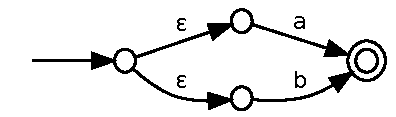
\includegraphics{filters/capturing_under_parenthesis1.pdf}
    \label{fig:capt_paren1}
  }
  \subfigure[\textsf{(a)(b)}]{
    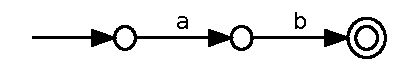
\includegraphics{filters/capturing_under_parenthesis2.pdf}
    \label{fig:capt_paren2}
  }
  \subfigure[\textsf{(?:\textbar (a))(?:\textbar (b))}]{
    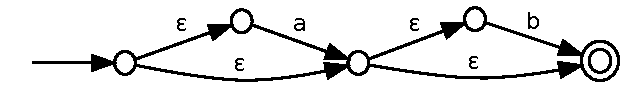
\includegraphics{filters/capturing_under_parenthesis3.pdf}
    \label{fig:capt_paren3}
  }
\caption{Capturing under alternation}
\end{figure}

\begin{example}[Capturing under alternation]
  \label{ex:capturing_under_alternation}
  In matching the regular expression \textsf{(a)\textbar (b)}, see
  figure \vref{fig:capt_paren1} for the NFA, with the string
  \textsl{a} we obtain these mixed bit-values: 
  \begin{center}\texttt{=0:1|t:b}\end{center}
  What these mixed bit-values are saying is that we have 2 channels,
  one that go through \textsf{a} and succeeds and one that go through
  \textsf{b} and fails. The succeeding channel never goes through
  \textsf{b}, the contents of that group is not defined.
  
  Rewriting the regular expression \textsf{(a)\textbar (b)} according
  to $G'$ we have:
  \begin{align*}
    G'[[\text{\textsf{(a)\textbar (b)}}]] &=
    G'[[\text{\textsf{(a)}}]]G'[[\text{\textsf{(b)}}]] \\
    &= \text{\textsf{(a)}}\text{\textsf{(b)}} \\
  \end{align*}
  In this regular expression there is only one way: The one going
  through both the groups. See figure \vref{fig:capt_paren2} for the
  NFA of the expression. This is bad news for our rewriting function
  and our filter, since we need some way of skipping groups: Each
  channel goes through only one group.
\end{example}

In example \ref{ex:capturing_under_alternation} we saw an example of
how undefined groups are not handled. To solve this problem we need
some way of signaling if a group participates in a match or not. We
define a new rewriting function $G''$ it is identical to $G'$ except
for equation \ref{eq:G1_paren} which is changed to:
\begin{align}
    G''[[(r)]] &= (?:|(r)) \notag
\end{align}
This change will enable us to choose which groups participates in a
match. This comes at a cost: Extra bits will have to be added to the
mixed bit-values output and extra alternations to the rewritten
regular expression. 

\begin{example}[continues=ex:capturing_under_alternation]
With the changed equation \ref{eq:G1_paren} we can continue our
example from before. Again we rewrite regular expression
\textsf{(a)\textbar (b)}, this time according to $G''$:
  \begin{align*}
    G''[[\text{\textsf{(a)\textbar (b)}}]] &=
    G''[[\text{\textsf{(a)}}]]G''[[\text{\textsf{(b)}}]] \\
    &= \text{\textsf{(?:\textbar (a))(?:\textbar (b))}} \\
  \end{align*}
  See figure \vref{fig:capt_paren3} for the NFA. As is clear from the
  rewritten regular expression and the NFA, there is now a way around
  the groups. Taking this into account, the output for the groupings
  filter should be: 
  \begin{center}\texttt{=1:01|0t:b}\end{center}
  What these mixed bit-values are saying is that we have two channels,
  one picks the route through \textsf{a}, around \textsf{b} and
  succeeds and the other picks the route around \textsf{a}, through
  \textsf{b} and fails.
\end{example}
As needed, we now have a way of signaling if a particular group is in
a match: Insert a 1 in the mixed bit-values and the group participates
or insert a 0 and it does not. 


\paragraph{Capturing under repetition}
The other problem we hinted at has to do with capturing under
repetition. When using a capturing subpattern, it can match repeatedly
using a quantifier. For example matching \textsf{(.)*} with the string
\textsl{abc}, the first time we apply the \textsf{*} we capture a
\textsl{a} the second time a \textsl{b} and the last time a
\textsl{c}. In such a case we have several options when reporting the
strings that was captured:
\begin{itemize}
\item The first
\item The last, this is the what most backtracking engines like Perl
  do
\item All, this is what a full regular expression engine do
\end{itemize}
Only two of these options are available to a streaming filter: All and
the first. In order to return the last match, we would have to save
the latest match when matching with the quantifier, it is potentially
the last and we can not know until we are done matching with the
quantifier.

Returning the first string that was captured by the quantifier, forces
us to throw away mixed bit-values generated in a capturing
parenthesis. We would only need the mixed bit-values generated by the
first iteration of the quantifier. 

To return all the strings captured by a group, we simply output all
the mixed bit-values generated while in the capturing
parenthesis. However, this causes problems with the rewriting
function. Rewriting \textsf{(.)*} according to $G''$ we have
\textsf{(.)}. This regular expression accepts one single character. In
no way can we make mixed bit-values, fitting this regular expression,
that represent a list of matched strings. Therefore we add the
following equations:
\begin{align*}
  G''[[(r)*]] &= (r)* \\
  G''[[(r)+]] &= (r)+
\end{align*}
We should now also keep the mixed bit-values that glues the iterations
together, even though they are outside the capturing group.




%% \begin{example}[Capturing under repetition]
%%   %% \begin{figure}
%%   %%   \centering
%%   %%   \subfigure[\textsf{(a)*}]{
%%   %%     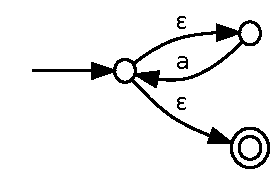
\includegraphics{filters/capt_under_rep1.pdf}
%%   %%     \label{fig:capt_rep1}
%%   %%   }
%%   %%   \subfigure[\textsf{(a)}]{
%%   %%     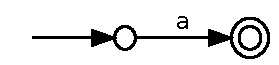
\includegraphics{filters/capt_under_rep2.pdf}
%%   %%     \label{fig:capt_rep2}
%%   %%   }
%%   %%   \caption{Capturing under repetition}
%%   %% \end{figure}

%%   %% In this example we will be matching regular expression
%%   %% \textsf{(a)*}, see figure \vref{fig:capt_rep1} for the NFA, with the
%%   %% string \textsl{aaa}. This match generates the following mixed
%%   %% bit-values:
%%   %% \begin{center}\texttt{=0:1|=0:1:b|=0:1:b|=0b:1t:b}\end{center}

%%   %% Rewriting \textsf{(a)*} according to $G''$ gives us:
%%   %% \begin{align*}
%%   %%   G''[[\text{\textsf{(a)*}}]] &= G''[[\text{\textsf{(a)}}]] \\
%%   %%   &= \text{\textsf{(a)}}
%%   %% \end{align*}
%%   %% See figure \vref{fig:capt_rep2} for the NFA.

%%   %% This rewrite works if we are only interested in one 

%%   By matching
%% \end{example}


%% To return all we need to make some changes to the rewriting function,
%% we add the following equations:
%% \begin{align*}
%%   G''[[(r)*]] &= (r)* \\
%%   G''[[(r)+]] &= (r)+
%% \end{align*}


%% We should not just throw away everything

%% If we choose to return all, all we need to do is add equations to the
%% rewriting function:
%% \begin{align*}
%%   G''[[(r)*]] &= (r)* \\
%%   G''[[(r)+]] &= (r)+
%% \end{align*}



%% Returning all would be the easier solution. We need to be careful when
%% rewriting the regular expression however. With the output from the
%% groupings filter we should be able to navigate the NFA for the
%% rewritten regular expression.


%% Returning all would be the easiest solution, this would however
%% require a change in the rewriting function. We add the equations:
%% \begin{align*}
%%   G''[[(r)*]] &= (r)* \\
%%   G''[[(r)+]] &= (r)+
%% \end{align*}


%% %% Returning all of the strings that were captured is by far the easiest,
%% %% no extra work is required. On the other hand if we only want to return
%% %% the first of the matches, we need to know whether or not to return a
%% %% particular match, that is if this is the first time we match with the
%% %% quantifier or not. If we alter the way we construct the NFA, we can
%% %% achieve this. 





%% \todo{Hvad den blippen er det nu for en løsning jeg har på det
%%   problemos}



We are now ready to present the final rewriting function: Definition
\vref{def:G}.
\begin{definition}[The groupings filter rewriting function]
  \label{def:G}
  For regular expressions $r$, $r_1$, $r_2$, defined over alphabet
  $\Sigma$, and $a$, any character from $\Sigma$, let $G$ be defined by:
  \begin{align*}
    G[[\upvarepsilon]] &= \upvarepsilon \\
    G[[a]] &= \upvarepsilon \\
    G[[ [...] ]] &= \upvarepsilon \\
    G[[r_1r_2]] &= G[[r_1]]G[[r_2]] \\
    G[[r_1|r_2]] &= G[[r_1]]G[[r_2]] \\
    G[[r*]] &= G[[r]] \\
    G[[r+]] &= G[[r]] \\
    G[[r?]] &= G[[r]] \\
    G[[(?:r)]] &= G[[r]] \\
    G[[(r)]] &= (?:|(E)) \\
    G[[(r)*]] &= (?:|(r)*) \\
    G[[(r)+]] &= (?:|(r)+) \\
  \end{align*}
\end{definition}
\begin{example}
  Here follows a few examples of how the groupings filter rewriting
  function, $G$, works.
  \begin{align*}
    G[[\mathsf{(a)|b}]] &= G[[\mathsf{(a)}]]G[[\mathsf{b}]]\\
    &= \mathsf{(?:(a))} \upvarepsilon\\
    &= \mathsf{(?:(a))}
  \end{align*}

  \begin{align*}
    G[[\mathsf{((cup)cake)}]] &= \mathsf{(?:|((cup)cake))}
  \end{align*}

  \begin{align*}
    G[[\mathsf{(a|b)*}]] &= \mathsf{(a|b)*}
  \end{align*}
\end{example}

